\documentclass[aspectratio=169]{beamer}
\usepackage[utf8]{inputenc}
\usepackage[T1]{fontenc}
\usepackage{listings}
\usepackage{lmodern}
\usepackage{tikz}
\usepackage{textpos} 
\usepackage{eurosym}
\usepackage{amsmath}
\usetikzlibrary{shapes,arrows,graphs,fit,backgrounds,matrix}
\definecolor{UniversityBlue}{RGB}{0, 81, 158}

\title{Lokale Operatoren / Laplace-Operator}
\date{16. Januar 2019}
\author{Medizintechnik - Marvin Banse}

\tikzstyle{block} = [draw, rectangle, text width=2cm, text centered, minimum height=1cm, node distance=3cm,fill=white]
\tikzstyle{container} = [draw, rectangle, inner sep=0.3cm, fill=gray,minimum height=2.5cm]
\def\bottom#1#2{\hbox{\vbox to #1{\vfill\hbox{#2}}}}
\tikzset{
  mybackground/.style={execute at end picture={
      \begin{scope}[on background layer]
        \node[] at (current bounding box.north){\bottom{1cm} #1};
        \end{scope}
    }},
}

\tikzset{
  treenode/.style = {align=center, inner sep=0pt, text centered,
    font=\sffamily},
  arn/.style = {treenode, circle, black, draw=black,
    text width=1.5em},% arbre rouge noir, noeud noir
  arn_r/.style = {treenode, circle, black, draw=black, 
    text width=1.5em},% arbre rouge noir, noeud rouge
  arn_x/.style = {treenode, rectangle, draw=black,
    minimum width=0.5em, minimum height=0.5em}% arbre rouge noir, nil
}

\newcommand{\setstdlayout}{
    \setbeamercolor{frametitle}{fg=white,bg=UniversityBlue}
    \addtobeamertemplate{frametitle}{}{%
        \begin{textblock*}{100mm}(.85\textwidth,-1cm)
            
\includegraphics[height=.11\textheight]{img/Uniol_1c_WEISS.eps}
        \end{textblock*}
    }
}

\newcommand{\setfoot}{
\setbeamertemplate{footline}{%
    \raisebox{8pt}{%
        \makebox[\paperwidth]{%
            \makebox[30pt]{}
            \footnotesize 
            
            % Titel für die Fußzeile
            
            \hfill\makebox[30pt]{%
                \footnotesize\insertframenumber/\inserttotalframenumber
            }
        }
    }
}
}
\newcommand{\clearfoot}{
    \setbeamertemplate{footline}{ }
}

\titlegraphic{
    
\includegraphics[height=.15\textheight]{img/Uniol_Cmyk.eps}
    \hfill
    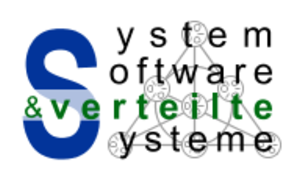
\includegraphics[height=.15\textheight]{img/logo_svs.eps}
}

\usetheme{metropolis}


\begin{document}


\clearfoot{ }
\setstdlayout{ }

\begin{frame}
    \titlepage
\end{frame}

\setfoot{}

\begin{frame}
    \frametitle{Definition}
    \begin{center}
    \begin{alertblock}
        {Lokaler Operator}
    \begin{itemize}
        \item In Form einer 3x3-Matrix \textit{(auch Template)}
        \item Berechnung eines Grauwerts g' an der Stelle (x,y)
        \item Berechnung Grauwerte an den Stellen (x+[-1:1],y+[-1:1]) \textit{(x,y)+Nachbarn)}
        \item Grauwerte am Rand werden gesondert betrachtet
    \end{itemize}
    \end{alertblock}
    \begin{alertblock}
        {Lokaler Filter}
        \begin{itemize}
            \item Anwendung eines Lokalen Operators auf jeden Eintrag einer Grauwertmatrix
            \item Die neuen Grauwerte werden in eine separate Matrix geschrieben 
            \item $\rightarrow$ Vermeidung von linearen Abhängigkeiten
        \end{itemize}
    \end{alertblock}
\end{center}
\end{frame}

\begin{frame}
    \frametitle{Definition}
    \begin{center}
    \begin{alertblock}
        {Mittelwert-Operator}
        \begin{equation}
            g'(x,y)=\sum_{i=-n/2}^{n/s}\sum_{j=-m/2}^{m/s}meanOp(x+j+1,y+i+1)*g(x+j,y+i)
        \end{equation}
        Template:
        \begin{equation}
            \frac{1}{9} *
            \begin{pmatrix}
                1 & 1 & 1 \\
                1 & 1 & 1 \\
                1 & 1 & 1 \\
            \end{pmatrix}
            =
            \begin{pmatrix}
                \frac{1}{9} & \frac{1}{9} & \frac{1}{9} \\
                \frac{1}{9} & \frac{1}{9} & \frac{1}{9} \\
                \frac{1}{9} & \frac{1}{9} & \frac{1}{9} \\
            \end{pmatrix}
        \end{equation}
    \end{alertblock}
    \begin{alertblock}
        {Mittelwertfilter}
        \begin{itemize}
            \item Anwendung des Mittelwert-Operators auf jeden Eintrag einer Grauwertmatrix
            \item Über den Rand hinaus wird ein Grauwert von 0 angenommen
            \item Schärfereduktion, Rauschfilterung
        \end{itemize}
    \end{alertblock}
    \end{center}
\end{frame}

\begin{frame}
    \frametitle{Beispiel: Mittelwertoperator}
    \begin{alertblock}
        {Angewendet an der Stelle (2,2) der Matrix M}
    \begin{center}
        \begin{equation} M =
            \begin{pmatrix}
                 2 &  2 &  3 &  4\\
                 5 &  6 &  7 &  8\\
                 9 & 10 & 11 & 12\\
                13 & 14 & 15 & 16\\
            \end{pmatrix}
            \rightarrow 
            \begin{pmatrix}
                2*\frac{1}{9} &  2*\frac{1}{9} &  3*\frac{1}{9} &  4\\
                 5*\frac{1}{9} &  6*\frac{1}{9} &  7*\frac{1}{9} &  8\\
                 9*\frac{1}{9} & 10*\frac{1}{9} & 11*\frac{1}{9} & 12\\
                13 & 14 & 15 & 16\\
            \end{pmatrix}
            \rightarrow
            \begin{pmatrix}
                \frac{2}{9} &  \frac{2}{9} &  \frac{3}{9}\\
                \frac{5}{9} &  \frac{6}{9} &  \frac{7}{9}\\
                 \frac{9}{9} & \frac{10}{9} & \frac{11}{9}\\
            \end{pmatrix}
        \end{equation}
        \begin{equation}
        \begin{aligned}
            g'(2,2) =\sum_{i=-1}^{1}\sum_{j=-1}^{1}meanOp(x+j+1,y+i+1)*g(x+j,y+i) \\
            = \frac{2}{9} + \frac{2}{9} + \frac{3}{9} + \frac{5}{9} + \frac{6}{9} + \frac{7}{9} + \frac{9}{9} + \frac{10}{9} + \frac{11}{9} = \frac{55}{9} = 6,\overline{1} \rightarrow 6
        \end{aligned}
        \end{equation}
    \end{center}
    \end{alertblock}
\end{frame}


\begin{frame}
    \frametitle{Aufgabe: Wenden Sie den 3x3-Mittelwertfilter auf das Bild an}
\begin{columns}
    \begin{column}{0.5\textwidth}
    \begin{alertblock}
        {Ungefilter:}
        \begin{footnotesize}
        \begin{equation*}
            \begin{pmatrix}
                5 &  2 &  6 &  2 &  3 &  2 &  1 &  2 &  3 &  1 \\
                1 &  3 &  6 &  7 &  9 &  2 &  4 &  4 &  7 &  1 \\
                1 &  5 &  8 &  8 & 10 & 17 & 21 & 19 &  9 &  4 \\
                4 & 18 & 34 & 56 & 17 & 25 & 38 & 17 &  7 &  2 \\
                1 & 14 & 22 & 43 & 68 & 91 & 62 & 23 & 16 &  7 \\
                6 & 12 & 21 & 21 & 39 & 87 & 76 & 34 &  4 &  2 \\
                9 & 24 & 54 & 73 & 88 & 95 & 69 & 16 & 12 &  5 \\
                3 &  5 &  6 & 40 & 34 & 42 &  6 &  4 &  2 &  5 \\
                4 &  9 & 16 & 14 & 32 & 51 & 13 &  6 &  6 &  2 \\
                4 &  2 &  5 & 3  &  3 &  3 &  5 &  3 &  3 &  3 \\
            \end{pmatrix}
        \end{equation*}
        \end{footnotesize}
    \end{alertblock}
    \end{column}
    \begin{column}{0.5\textwidth}
    \begin{alertblock}
        {Mittelwertgefiltert:}
        \begin{footnotesize}
        \begin{equation*}
            \begin{pmatrix}
                1 &  2 &  2 &  3 &  2 &  2 &  1 &  2 &  2 &  1 \\
                1 &  4 &  5 &  6 &  6 &  7 &  8 &  7 &  5 &  2 \\
                3 &  8 & 16 & 17 & 16 & 15 & 16 & 14 &  7 &  3 \\
                4 & 11 & 23 & 29 & 37 & 38 & 34 & 23 & 11 &  5 \\
                6 & 14 & 26 & 35 & 49 & 55 & 50 & 30 & 12 &  4 \\
                7 & 18 & 31 & 47 & 67 & 75 & 61 & 34 & 13 &  5 \\
                6 & 15 & 28 & 41 & 57 & 59 & 47 & 24 &  9 &  3 \\
                6 & 14 & 26 & 39 & 52 & 47 & 33 & 14 &  6 &  3 \\
                3 &  6 & 11 & 17 & 24 & 21 & 14 &  5 &  3 &  2 \\
                2 &  4 &  5 &  8 & 11 & 11 &  9 &  4 &  2 &  1 \\
            \end{pmatrix}
        \end{equation*}
        \end{footnotesize}
    \end{alertblock}
    \end{column}
    \end{columns}
\end{frame}

\begin{frame}
    \frametitle{Aufgabe: Wenden Sie den 3x3-Mittelwertfilter auf das Bild an}
\begin{columns}
    \begin{column}{0.5\textwidth}
    \begin{alertblock}
        {Ungefilter:}
        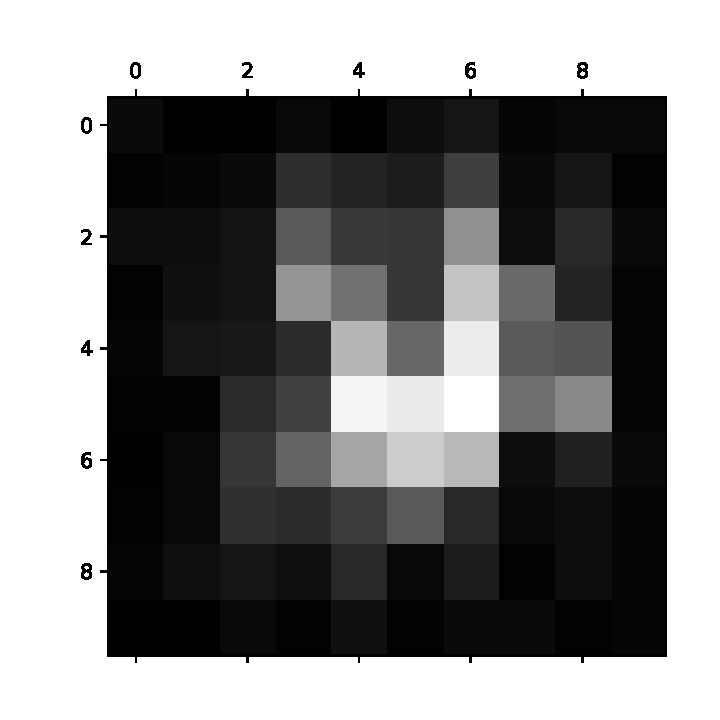
\includegraphics[width=1\textwidth]{../raw.pdf}
    \end{alertblock}
    \end{column}
    \begin{column}{0.5\textwidth}
    \begin{alertblock}
        {Mittelwertgefiltert:}
        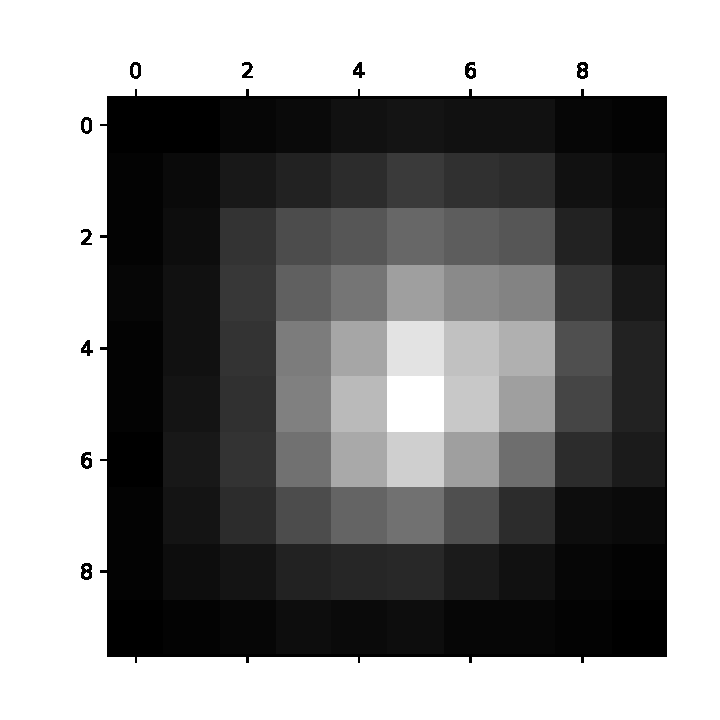
\includegraphics[width=1\textwidth]{../mean.pdf}
    \end{alertblock}
    \end{column}
    \end{columns}
\end{frame}

\begin{frame}
    \frametitle{Aufgabe: Begründen Sie die Wahl des Umgangs mit Randpixeln}
    \begin{alertblock}
        {Vorgehen}
        \begin{equation}
            g'(0,0) = \frac{0+0+0+0+5+2+0+1+3}{9} = \frac{11}{9} = 1,22 = 1
        \end{equation}
    \end{alertblock}
    \begin{alertblock}
        {Begründung}
        \begin{itemize}
            \item Für den Raum um das Objekt wird Luft angenommen $\rightarrow$ schwarz $\rightarrow$ 0
            \item Abhängig von der Umgebung können andere Grauwerte angenommen werden (z.B. 100)
        \end{itemize}
    \end{alertblock}
\end{frame}

\begin{frame}
    \frametitle{Definition}
    \begin{center}
    \begin{alertblock}
        {Laplace-Operator}
        \begin{equation}
            g'(x,y)=\sum_{i=-n/2}^{n/s}\sum_{j=-m/2}^{m/s}laplaceOp(x+j+1,y+i+1)*g(x+j,y+i)
        \end{equation}
        Template:
        \begin{equation}
            \begin{pmatrix}
                0 &  1 & 0 \\
                1 & -4 & 1 \\
                0 &  1 & 0 \\
            \end{pmatrix}
        \end{equation}
    \end{alertblock}
    \begin{alertblock}
        {Skalierbarer Laplace-Operator}
        Template:
        \begin{equation}
            \begin{pmatrix}
                0 & 0 & 0 \\
                0 & 1 & 0 \\
                0 & 0 & 0 \\
            \end{pmatrix} - \epsilon *
            \begin{pmatrix}
                0 &  1 & 0 \\
                1 & -4 & 1 \\
                0 &  1 & 0 \\
            \end{pmatrix} = 
            \begin{pmatrix}
                0 &  -\epsilon & 0 \\
                -\epsilon & 1+4\epsilon & -\epsilon \\
                0 &  -\epsilon & 0 \\
            \end{pmatrix} 
        \end{equation}
    \end{alertblock}
    \end{center}
\end{frame}

\begin{frame}
    \frametitle{Beispiel: Laplace-Operator}
    \begin{alertblock}
        {Angewendet an der Stelle (2,2) der Matrix M}
    \begin{center}
        \begin{equation} M =
            \begin{pmatrix}
                 2 &  2 &  3 &  4\\
                 5 &  6 &  7 &  8\\
                 9 & 10 & 11 & 12\\
                13 & 14 & 15 & 16\\
            \end{pmatrix}
            \rightarrow 
            \begin{pmatrix}
                 2*0 &  2*1  &  3*0 &  4\\
                 5*1 &  6*-4 &  7*1 &  8\\
                 9*0 & 10*1  & 11*0 & 12\\
                13 & 14 & 15 & 16\\
            \end{pmatrix}
            \rightarrow
            \begin{pmatrix}
                0 &   2 &  0\\
                5 & -24 &  7\\
                0 &  10 &  0\\
            \end{pmatrix}
        \end{equation}
        \begin{equation}
        \begin{aligned}
            g'(2,2) =\sum_{i=-1}^{1}\sum_{j=-1}^{1}laplaceOp(x+j+1,y+i+1)*g(x+j,y+i) \\
            = 0+2+0+5-24+7+10 = 0
        \end{aligned}
        \end{equation}
    \end{center}
    \end{alertblock}
\end{frame}

\begin{frame}
    \frametitle{Aufgabe: Berechnen Sie die Kontur der Objekte}
\begin{columns}
    \begin{column}{0.4\textwidth}
    \begin{alertblock}
        {Ungefilter:}
        \begin{tiny}
        \begin{equation*}
            \begin{pmatrix}
                5 &  2 &  6 &  2 &  3 &  2 &  1 &  2 &  3 &  1 \\
                1 &  3 &  6 &  7 &  9 &  2 &  4 &  4 &  7 &  1 \\
                1 &  5 &  8 &  8 & 10 & 17 & 21 & 19 &  9 &  4 \\
                4 & 18 & 34 & 56 & 17 & 25 & 38 & 17 &  7 &  2 \\
                1 & 14 & 22 & 43 & 68 & \textcolor{red}{91} & 62 & 23 & 16 &  7 \\
                6 & 12 & 21 & 21 & 39 & 87 & 76 & 34 &  4 &  2 \\
                9 & 24 & 54 & 73 & 88 & 95 & 69 & 16 & 12 &  5 \\
                3 &  5 &  6 & 40 & 34 & 42 &  6 &  4 &  2 &  5 \\
                4 &  9 & 16 & 14 & 32 & 51 & 13 &  6 &  6 &  2 \\
                4 &  2 &  5 & 3  &  3 &  3 &  5 &  3 &  3 &  3 \\
            \end{pmatrix}
        \end{equation*}
        \end{tiny}
    \end{alertblock}
    \end{column}
    \begin{column}{0.6\textwidth}
    \begin{alertblock}
        {Laplacegefiltert:}
        \begin{tiny}
        \begin{equation*}
            \begin{pmatrix}
                 -17 &   6 & -14 &    8 &    1 &   -2 &   4 &   0 &  -2 &   0 \\
                   5 &   2 &   0 &   -3 &  -14 &   24 &  12 &  16 & -11 &   8 \\
                   6 &  10 &  21 &   49 &   11 &  -10 &  -6 & -25 &   1 &  -4 \\
                   4 & -15 & -32 & -122 &   91 &   63 & -27 &  19 &  16 &  10 \\
                   20 &  -3 &  24 &   -5 &  -82 & \textcolor{red}{-122} & -20 &  37 & -23 &  -8 \\
                  -2 &  17 &  25 &   92 &  108 &  -47 & -52 & -17 &  48 &   8 \\
                  -3 & -16 & -92 &  -89 & -111 &  -94 & -83 &  55 & -21 &  -1 \\
                   6 &  22 &  91 &  -33 &   66 &   18 & 104 &  14 &  19 & -11 \\
                   0 &  -9 & -30 &   35 &  -26 & -114 &  16 &   2 & -11 &   6 \\
                 -10 &  10 &   1 &   10 &   26 &   47 &  -1 &   2 &   0 &  -7 \\
            \end{pmatrix}
        \end{equation*}
        \end{tiny}
    \end{alertblock}
    \end{column}
    \end{columns}
    \begin{alertblock}
        {Größte Grauwertänderung:}
        213 an der Stelle (5,6)
    \end{alertblock}
\end{frame}

\begin{frame}
    \frametitle{Aufgabe: Berechnen Sie die Kontur der Objekte}
\begin{columns}
    \begin{column}{0.5\textwidth}
    \begin{alertblock}
        {Ungefilter:}
        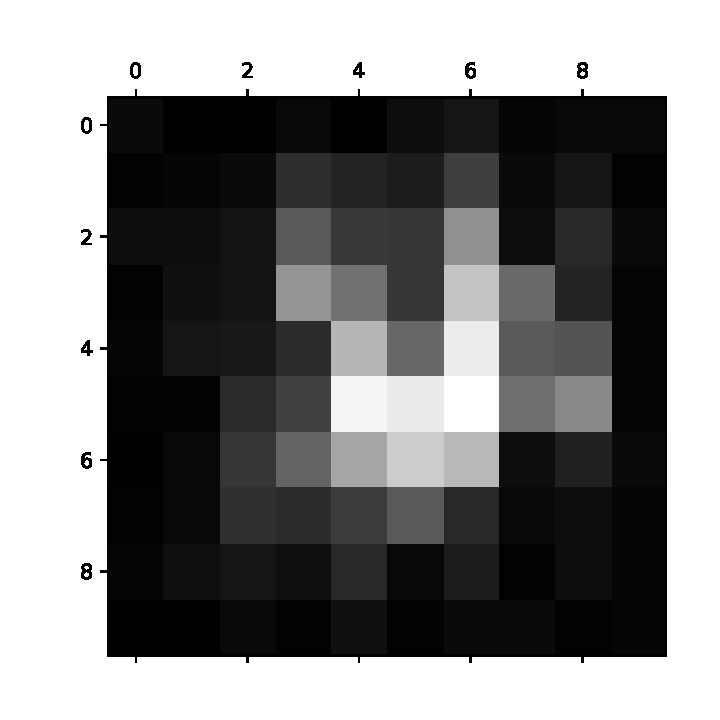
\includegraphics[width=1\textwidth]{../raw.pdf}
    \end{alertblock}
    \end{column}
    \begin{column}{0.5\textwidth}
    \begin{alertblock}
        {Laplacegefiltert:}
        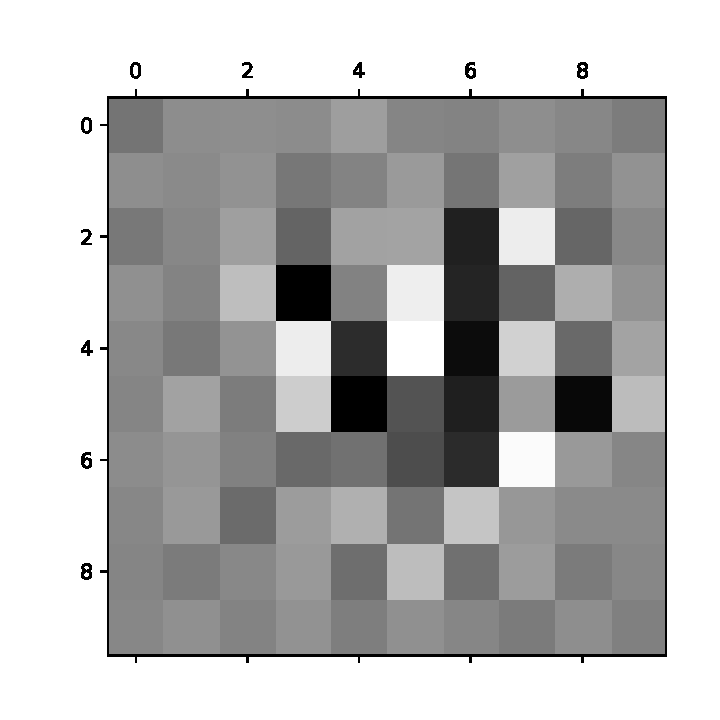
\includegraphics[width=1\textwidth]{../laplace.pdf}
    \end{alertblock}
    \end{column}
    \end{columns}
\end{frame}

\end{document}
